\documentclass[journal,twocolumn]{IEEEtran}

\usepackage{amsmath,amssymb}
\usepackage{graphicx}
\usepackage{booktabs}
\usepackage{tikz}
\usetikzlibrary{arrows.meta,positioning,calc,fit,backgrounds}
\usepackage{url}
\usepackage[caption=false,font=footnotesize]{subfig}

% ---- data macros: every number below is produced by the released scripts ----
\newcommand{\NMAC}{8}
\newcommand{\DWID}{16}
\newcommand{\PART}{xc7a100tcsg324-1}

\begin{document}

\title{Composable Sparsity Gating for\\Completion-Aware Clock-Gated MAC Arrays}

\author{Kulamani~Rout% <-- AFFILIATION PLACEHOLDER
\thanks{The author is with [AFFILIATION TO BE SUPPLIED]
(e-mail: routsarojini901@gmail.com).}
\thanks{Design sources, testbenches and the complete Vivado build/power
scripts needed to reproduce every number in this brief are released with
the paper.}}

\markboth{IEEE TRANSACTIONS ON CIRCUITS AND SYSTEMS--II: EXPRESS BRIEFS}%
{Rout: Composable Sparsity Gating for Completion-Aware Clock-Gated MAC Arrays}

\maketitle

\begin{abstract}
Operand zero-skipping and completion-aware clock gating are both established
low-power techniques for multiply--accumulate (MAC) arrays, and are routinely
described as complementary. This brief shows that they are not directly
composable. Wherever a single clock enable is shared between the operation arriving this
cycle and operations already in flight---the normal case for stage-level
gating---the widely used sparsity enable
$\mathrm{EN}=\mathit{valid}\wedge(A\neq0)\wedge(B\neq0)$ silently applies one operation's
condition to its predecessors. With completion-aware (drain-counter) gating
the consequence is deterministic rather than intermittent, because a correctly
sized drain window has zero slack by construction and the stranded result is
never produced. On an
eight-lane cascaded MAC array this drops \textbf{63\,\% of all results}. We
give a structural fix---splitting the clock enable into a never-masked control
enable and a sparsity-gated datapath enable, with the skip decision carried
per item---and prove it cycle-for-cycle equivalent to the ungated reference
over randomised sparse traffic, using the broken design as a negative control.
We further show that register-enable activity counts, the metric usually
quoted for such schemes, materially overstate the saving, and that an
asynchronous datapath reset silently prevents the DSP48 register packing on
which the real saving depends.
\end{abstract}

\begin{IEEEkeywords}
Clock gating, sparsity, multiply--accumulate, low-power design, FPGA,
design verification.
\end{IEEEkeywords}

\section{Introduction}
\IEEEPARstart{D}{ynamic} power in a MAC array is dominated by the multiplier
array and its pipeline registers. Two mitigations are standard. \emph{Clock
gating} suppresses register activity while a stage is idle
\cite{benini,wupedram}. \emph{Zero-skipping} exploits the high operand
sparsity of quantised CNN inference: because $a=0 \vee b=0 \Rightarrow ab=0$
exactly, the multiply may be skipped without any loss of accuracy. Zero-skip
has been used at architectural scale in Eyeriss \cite{eyeriss}, Cnvlutin
\cite{cnvlutin}, SCNN \cite{scnn} and EIE \cite{eie}, is claimed in industrial
patents \cite{pat_google,pat_img}, and appears at RTL as the enable
\begin{equation}
\mathrm{EN}_{\mathrm{MAC}}=\mathit{valid}\wedge(A\neq0)\wedge(B\neq0)
\label{eq:naive}
\end{equation}
used, for example, in a recent FPGA power-optimisation study \cite{gohel}.

The two techniques are habitually presented as orthogonal: one removes idle
activity, the other removes ineffectual activity. This brief shows that the
orthogonality fails as soon as the clock gate is \emph{completion-aware}, that
is, when the enable is held asserted by a drain counter until every in-flight
pipeline slot has retired. The contributions are:

\begin{enumerate}
\item A demonstration that (\ref{eq:naive}) is unsafe in a drain-gated
pipeline, with the failure mechanism identified as the zero-slack property of
a correctly sized drain window (Section~\ref{sec:hazard}).
\item A split-enable construction that restores composability at negligible
cost, together with a lossless propagation of sparsity information into the
downstream adder tree (Section~\ref{sec:fix}).
\item An equivalence-based verification method that uses the broken design as
a negative control, so that the passing result is shown to be non-vacuous
(Section~\ref{sec:verif}).
\item Post-implementation evidence that register-enable activity counts,
the metric usually quoted for such schemes, can overstate the achievable
saving by the entire multiplier contribution, and that the resulting
correction is affordable only if the datapath reset style permits DSP
packing (Section~\ref{sec:results}).
\end{enumerate}

\section{Completion-Aware Gating Baseline}
\label{sec:baseline}
The reference design is an \NMAC-lane array of two-stage
(multiply, accumulate) \DWID-bit MACs feeding a three-level registered adder
tree. Each stage owns an independent gating cell parameterised by its own
pipeline depth $D$:
\begin{equation}
\mathit{ce}=\mathit{pe}\vee\mathit{oa}\vee\mathit{trig},
\label{eq:ce}
\end{equation}
where $\mathit{trig}$ marks the cycle a new item enters, $\mathit{oa}$ is a
registered ``operation active'' flag, and $\mathit{pe}$ is an external
override. On $\mathit{trig}$ a counter loads $D$; otherwise it decrements, and
$\mathit{oa}$ falls when it reaches zero. The disjunction with
$\mathit{trig}$ in (\ref{eq:ce}) is required because $\mathit{oa}$ is
registered and would otherwise drop the first cycle of every burst.

The array does not use a central controller. Stage~2 is triggered by the
disjunction of the lanes' completion outputs, so each stage independently
wakes its successor---the arrangement is a cascade of autonomous gates rather
than a scheduled pipeline. Related distributed pipeline gating is claimed in
\cite{pat_ibm}, which propagates stall and valid signals rather than
maintaining per-stage drain counters.

\section{The Composability Hazard}
\label{sec:hazard}

\subsection{Drain windows have zero slack}
A drain counter is correct when $D$ equals the stage latency: a smaller $D$
strands in-flight data, a larger one wastes enable cycles. Sizing it correctly
therefore makes the enable window exactly as long as the pipeline needs and
not one cycle longer. Measurement on the reference design confirms this. For a
single item entering at cycle $T$, the MAC's $\mathit{ce}$ is asserted only
during $\{T,T{+}1,T{+}2\}$, and $\mathit{completion\_out}$ fires in $T{+}2$,
the \emph{last} asserted cycle. The adder tree behaves identically over four
cycles. There is no spare enable cycle anywhere.

\subsection{Failure mechanism}
Consider a burst in which a zero-valued operand arrives at $T{+}1$, one cycle
after a non-zero item. Under (\ref{eq:naive}) the shared enable is deasserted
at $T{+}1$. That enable, however, is not private to the arriving item: it also
clocks the accumulate stage of the item that entered at $T$ and is mid-drain.
Suppressing it defers that accumulation; because the drain counter continues
to run regardless, the enable window closes before the deferred accumulation
can occur, and the result is lost permanently. The three canonical cases are
zero mid-burst, zero at burst start, and zero at burst end; only the last is
fatal, and only because of the zero-slack property.

The hazard is more general than the drain counter that exposes it. It arises
whenever a \emph{single} clock enable is shared between the item arriving in
the current cycle and items already in flight in the same stage---which is the
normal situation for stage-level gating, however the enable is generated.
Deriving that enable from a per-item condition such as (\ref{eq:naive}) then
silently applies one item's condition to its predecessors. What a correctly
sized drain counter changes is only that it removes the accidental slack which
might otherwise let the stranded operation catch up on a later idle cycle, and
so converts an intermittent, data-dependent fault into a deterministic one.
Schemes that hold the enable using a valid shift register, or a
\emph{busy}/\emph{stall} signal, share the same exposure.

\begin{figure}[t]
\centering
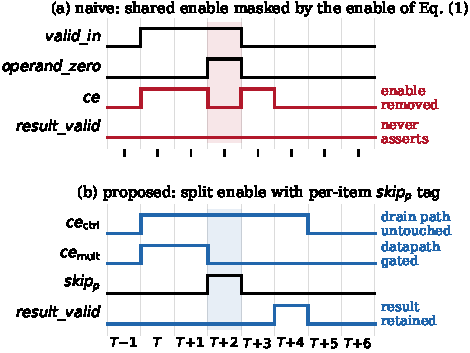
\includegraphics[width=\columnwidth]{fig_timing.pdf}
\caption{The composability hazard. A zero operand at $T{+}2$ lands inside the
drain window of the item that entered at $T{+}1$. (a) Masking the shared
enable strands that item; because the drain counter runs regardless, the
window closes and the result is never produced. (b) Splitting the enable
leaves the drain path untouched and gates only the datapath, so the result is
retained.}
\label{fig:timing}
\end{figure}

Fig.~\ref{fig:timing} contrasts the two cases. The effect is not marginal.
Implementing (\ref{eq:naive}) verbatim on the
reference cascade and comparing against the ungated design under identical
stimulus, the naive design produces \textbf{77 of 208} expected result
pulses---\textbf{63\,\% of results silently dropped}---and differs from the
reference on \textbf{278 of 284} compared cycles. It does not compute wrong
sums so much as stop computing.

\section{Split-Enable Zero-Skip}
\label{sec:fix}

\subsection{Construction}
The fix is to stop treating the clock enable as a single signal. We derive
\begin{align}
\mathit{skip} &= \mathit{valid}\wedge\left(\overline{|a}\;\vee\;\overline{|b}\right)\\
\mathit{ce}_{\mathrm{ctrl}} &= f_{\mathrm{drain}}(\mathit{trig}=\mathit{valid})\\
\mathit{ce}_{\mathrm{mult}} &= \mathit{ce}_{\mathrm{ctrl}}\wedge \mathit{valid}\wedge\overline{\mathit{skip}}\\
\mathit{ce}_{\mathrm{acc}}  &= \mathit{ce}_{\mathrm{ctrl}}\wedge \mathit{valid}_{p}\wedge\overline{\mathit{skip}_{p}}
\end{align}
Two properties matter. First, the drain counter is triggered by the
\emph{raw} $\mathit{valid}$ and is therefore structurally blind to sparsity:
no operand pattern can shorten, extend or corrupt it. Second, the skip
decision is registered alongside the item as $\mathit{skip}_p$, exactly
parallel to the validity tag $\mathit{valid}_p$, so the accumulate stage
consults the tag belonging to \emph{its own} item rather than whatever is on
the input bus in the current cycle. This is what makes the zero-at-burst-end
case safe: the arriving zero cannot suppress a predecessor's accumulation
because that predecessor carries $\mathit{skip}_p=0$.

Only the two wide register banks are sparsity-gated. The three control
flip-flops per lane remain ungated; gating them would require perturbing
completion timing, which the zero-slack window forbids, and they represent
under 5\,\% of the lane's registers.

\subsection{Hierarchical propagation}
Per-lane skipping is local. The cascade admits a stronger statement: if a
lane's accumulator did not change, every partial sum in the tree that depends
only on unchanged accumulators is also unchanged and its register may be held.
Each lane exports $\mathit{upd}$ (``my accumulator moved''), registered in the
same cycle as its completion output, from which
\begin{equation}
\mathit{en}^{(1)}_{j}=\mathit{upd}_{2j}\vee \mathit{upd}_{2j+1},\quad
\mathit{en}^{(l+1)}_{k}=\mathit{chg}^{(l)}_{2k}\vee \mathit{chg}^{(l)}_{2k+1}
\end{equation}
with $\mathit{chg}^{(l)}$ the registered form of $\mathit{en}^{(l)}$, so that
the change flags advance up the tree in the same pipeline phase as the data
they describe. Holding a register whose inputs provably did not change is
bit-exact. Note the exploited property is \emph{unchangedness}, not zeroness:
the tree sums accumulators, which are persistent state and rarely zero. This
distinguishes the mechanism from operand-zero gating of adder trees
\cite{pat_img}. Under unstructured sparsity $s$ a level-1 adder idles only
when both feeding lanes idle, i.e.\ with probability $s^2$; the measured
level-1 and level-2 savings at $s=0.48$ are 22.7\,\% and 4.9\,\% against
$s^2=23\,\%$ and $s^4=5.3\,\%$ predicted. The tree contribution is therefore
genuinely second order and is reported as such.

\section{Verification}
\label{sec:verif}
Because zero-skip is lossless by construction, the gated and ungated designs
must agree on \emph{every} cycle, not merely at the end of a burst. Both are
driven from identical stimulus wires and compared cycle-for-cycle on
$(\mathit{result},\mathit{result\_valid})$; an independent behavioural model
of the per-lane accumulators is checked in parallel, so a fault corrupting
both designs identically would still be caught. Stimulus comprises eleven
directed cases covering the three canonical zero positions, all-zero bursts, a
twelve-cycle zero run with resumption, per-lane heterogeneous sparsity, and a
400-cycle randomised sparse stream.

A passing equivalence check proves nothing unless it can fail. We therefore
retain the naive design of Section~\ref{sec:hazard} as a \emph{negative
control} and run it in the same harness. Table~\ref{tab:verif} reports both.
The reference emits 208 result pulses, establishing non-vacuity; the proposed
design matches on every cycle; the naive design is caught.

\begin{table}[t]
\caption{Equivalence against the ungated reference}
\label{tab:verif}
\centering
\begin{tabular}{lccc}
\toprule
Design & result pulses & diverging cycles & verdict\\
\midrule
Reference (ungated)      & 208 & --- & ---\\
Proposed (split enable)  & 208 & 0 / 284 & pass\\
Naive, Eq.~(\ref{eq:naive}) & 77  & 278 / 284 & fail\\
\bottomrule
\end{tabular}
\end{table}

\section{Implementation Results}
\label{sec:results}
All designs were synthesised and implemented out of context on \PART{} with
Vivado 2023.2 at a 4.0\,ns target, budgeting 20\,\% of the period to off-core
delay on both inputs and outputs. Out-of-context implementation is
required---the cascade has 311 ports against 210 available pins---and is also
appropriate here because it excludes I/O buffer power from the comparison.
Timing every port path uniformly matters: false-pathing the inputs would
exclude the multiplier-input paths of the two-stage designs from analysis
altogether and render the frequency column meaningless. Power is obtained
from \texttt{report\_power} driven by SAIF activity captured from simulation
of the same LFSR stimulus, so every design sees bit-identical data at a given
sparsity. Table~\ref{tab:area} summarises area and timing.

\input{tab_area}

\subsection{The cost of composability}
The final two rows of Table~\ref{tab:area} differ only in whether sparsity gating is
enabled, and so isolate its true cost: \textbf{+117 LUT (+28\,\%) and +30 FF
(+10\,\%), with no frequency penalty} (283.0 against 271.7\,MHz). Applied
instead to the original two-stage pipeline (the two-stage rows) the split-enable
construction costs +101 LUT (+12.8\,\%) and +22 FF, again at no loss of
$F_{\max}$. Composability is therefore cheap; what is expensive is getting the
surrounding register style wrong, as the next two subsections show.

\subsection{Register-enable counts overstate the saving}
The two-stage split-enable design gates the \emph{product} register, and
activity counting there suggests a 64\,\% reduction in load events at 30\,\%
sparsity. Post-implementation this is misleading. Vivado maps each multiply to
a DSP48E1 but reports $\mathrm{AREG}=\mathrm{BREG}=\mathrm{MREG}=0$ with only
the product register absorbed ($\mathrm{PREG}=8$). The multiplier array is
consequently driven combinationally from whatever lies outside the DSP---here,
directly from the operand ports, which toggle every cycle irrespective of any
enable. Gating the product register saves that register's own load and
nothing of the array behind it.

Quieting the array requires \emph{gated operand} registers, so that a skipped
item leaves the DSP inputs unchanged. Measured at 29\,\% sparsity, transitions
at the multiplier inputs fall from 2661 to 1009, a 62\,\% reduction, whereas
the product-register-gated design scores \emph{zero} on the same metric. The
distinction is invisible to register-enable activity counting. We suggest that
where such counts are used to justify a gating scheme, the register being
gated should be stated explicitly, since gating a pipeline register downstream
of a combinational block does not quiet that block.

\subsection{Asynchronous reset blocks the fix}
Adding the operand registers in the design's existing house style---with
asynchronous reset---leaves them in fabric (third block of Table~\ref{tab:area}). The critical path becomes
a fabric flip-flop driving a DSP48 input pin with \emph{zero} logic levels and
predominantly route delay, missing the target by 0.94\,ns and costing 25\,\%
of $F_{\max}$, while register count rises by 272. The cause is that DSP48E1
A/B/M pipeline registers support only synchronous reset, so an asynchronously
reset register can never be absorbed into the slice. This constraint is
documented \cite{ug901} rather than new; what is worth reporting is that it is
\emph{decisive} for sparsity gating specifically. Gating an operand register is
the only way to quiet a combinational multiplier, so a house reset style that
merely costs area in an ordinary datapath here determines whether the entire
technique is affordable.

Removing the reset from the datapath registers---which do not require one,
since correctness is enforced by the validity and skip tags, and those
\emph{are} reset---restores full packing: $\mathrm{AREG}=\mathrm{BREG}=
\mathrm{MREG}=\mathrm{PREG}=8$ (final block). The accumulator's carry chain is
absorbed into the DSP's own adder as well, halving CARRY4 usage from 127 to
63. The two variants are cycle-for-cycle bit-identical over 3031 cycles and
2823 result pulses, so this is a coding-style change with no architectural
content---yet it decides whether the technique is affordable. The net outcome
is that the gated, DSP-packed cascade is \textbf{33\,\% smaller and 4.9\,\%
faster than the ungated baseline it replaces}, at the cost of one additional
cycle of latency.

\subsection{Power}
Table~\ref{tab:power} reports dynamic power at matched sparsity. Two
properties of the measurement deserve stating, because both are routinely
omitted.

First, \emph{the ungated baseline's own power falls with sparsity}: zero
operands toggle a multiplier array less regardless of any gating, and the
baseline drops 31\,\% between $s=0$ and $s=0.9$ with no gating whatsoever.
Comparing a gated design at high sparsity against an ungated one at $s=0$
therefore credits the gating with a reduction that is mostly a property of the
data. Each design here is compared against its own structural control at the
same sparsity. On that basis split-enable zero-skip costs 3\,\% at $s=0$---the
price of the detect and tag logic when there is no sparsity to exploit---and
returns 26\,\% at $s=0.75$ and 40\,\% at $s=0.9$.

Second, \emph{clock power is a floor}. No BUFGCE is inferred in any variant:
enable-based gating on this device maps to the flip-flops' native CE pins, not
to clock-tree gating. That component is 20\,mW in the baseline at every
sparsity---29\,\% of its dynamic power---and no technique in this class
removes it. A percentage saving quoted without stating this floor overstates
what is achievable on FPGA.

Separately, DSP packing alone reduces dynamic power from 70\,mW to 46\,mW at
$s=0$, consistent with the area reduction of Table~\ref{tab:area}. The
reset-style correction is thus worth more in absolute terms than the gating
itself, and the two are complementary rather than alternatives.

\begin{table}[t]
\caption{Dynamic power (mW) at matched operand sparsity}
\label{tab:power}
\centering\footnotesize
\setlength{\tabcolsep}{4.5pt}
\begin{tabular}{lcccc}
\toprule
Design & \multicolumn{4}{c}{operand sparsity $s$ (\%)}\\
\cmidrule(l){2-5}
 & 0 & 50 & 75 & 90\\
\midrule
Baseline (2-stage, async reset) & 70 & 65 & 58 & 48\\
\quad + split-enable zero-skip & 72 & 56 & 43 & 29\\
\quad\emph{change vs.\ its control} & \emph{+3\%} & \emph{-14\%} & \emph{-26\%} & \emph{-40\%}\\
\midrule
DSP-packed, gating off & 46 & 45 & 45 & 43\\
\quad + split-enable zero-skip & 47 & 45 & 41 & 37\\
\quad\emph{change vs.\ its control} & \emph{+2\%} & \emph{-0\%} & \emph{-9\%} & \emph{-14\%}\\
\midrule
clock component (baseline) & 20 & 20 & 20 & 20\\
\bottomrule
\end{tabular}
\\[2pt]
\raggedright\scriptsize Vivado \texttt{report\_power}; confidence Medium.
Each design is compared against its own structural control at the same
sparsity, because the ungated baseline itself loses 31\,\% of its power
between $s=0$ and $s=0.9$ from reduced multiplier switching alone.
The DSP-packed rows understate the gating benefit: see
Section~\ref{sec:results}-E.
\end{table}




\subsection{A limitation of SAIF-based comparison}
The DSP-packed rows of Table~\ref{tab:power} \emph{understate} the benefit of
gating, and we report them as a lower bound rather than a result. Applying an
RTL-simulation SAIF to a routed checkpoint annotated only 12--13\,\% of design
nets. For two designs of identical structure this is tolerable, because the
shortfall is common-mode; between the fabric-register and DSP-packed designs
it is not, because the gated operand registers of the latter are absorbed
\emph{into} the DSP48 slice and so have no corresponding net to annotate. The
symptom is unmistakable: the DSP power component of the packed design reads a
flat 20\,mW at every sparsity while the baseline's falls from 21\,mW to 7\,mW.
That flatness is an artefact of the annotation, not a property of the circuit.
Post-implementation netlist simulation is the standard remedy and did not
improve net matching in our attempts; resolving it is left as future work.

For that variant the two quantities independent of any power model are
therefore the more informative: the implementation data of
Table~\ref{tab:area}, and the direct switching measurement of
Section~\ref{sec:results}-B, in which multiplier-input transitions fall by
62\,\%.

\section{Conclusion}
Sparsity gating and completion-aware clock gating do not compose. The standard
zero-skip enable applied to a drain-gated MAC pipeline destroys 63\,\% of
results, and the reason---a correctly sized drain window has no slack---is
structural rather than incidental, so it will recur in any design combining
the two. Splitting the enable into a never-masked control enable and a
per-item-tagged datapath enable restores composability with no loss of
throughput and no change to completion timing. Two secondary results are of
independent interest: register-enable activity counts substantially overstate
the benefit of gating a multiplier's output register, and asynchronous
datapath resets silently prevent the DSP packing on which the genuine saving
depends.

\begin{thebibliography}{99}
\bibitem{benini} L.~Benini and G.~De~Micheli, ``Automatic synthesis of
low-power gated-clock finite-state machines,'' \emph{IEEE Trans.
Comput.-Aided Design Integr. Circuits Syst.}, vol.~15, no.~6, pp.~630--643,
Jun.~1996.

\bibitem{wupedram} Q.~Wu, M.~Pedram, and X.~Wu, ``Clock-gating and its
application to low power design of sequential circuits,'' \emph{IEEE Trans.
Circuits Syst.~I, Fundam. Theory Appl.}, vol.~47, no.~3, pp.~415--420,
Mar.~2000.

\bibitem{eyeriss} Y.-H. Chen, T.~Krishna, J.~S. Emer, and V.~Sze, ``Eyeriss:
An energy-efficient reconfigurable accelerator for deep convolutional neural
networks,'' \emph{IEEE J. Solid-State Circuits}, vol.~52, no.~1, pp.~127--138,
Jan.~2017.

\bibitem{cnvlutin} J.~Albericio, P.~Judd, T.~Hetherington, T.~Aamodt,
N.~E. Jerger, and A.~Moshovos, ``Cnvlutin: Ineffectual-neuron-free deep neural
network computing,'' in \emph{Proc. ACM/IEEE Int. Symp. Comput. Archit.
(ISCA)}, 2016, pp.~1--13.

\bibitem{scnn} A.~Parashar \emph{et al.}, ``SCNN: An accelerator for
compressed-sparse convolutional neural networks,'' in \emph{Proc. ACM/IEEE
Int. Symp. Comput. Archit. (ISCA)}, 2017, pp.~27--40.

\bibitem{eie} S.~Han \emph{et al.}, ``EIE: Efficient inference engine on
compressed deep neural network,'' in \emph{Proc. ACM/IEEE Int. Symp. Comput.
Archit. (ISCA)}, 2016, pp.~243--254.

\bibitem{gohel} D.~Gohel, A.~Gundrapally, and K.~Choi, ``RTL-level power
optimization of CNN accelerators via clock gating and sparsity-aware MAC
suppression on FPGA,'' \emph{Electronics}, vol.~15, no.~11, art.~2492, 2026.

\bibitem{pat_google} O.~Temam \emph{et al.}, ``Exploiting input data sparsity
in neural network compute units,'' U.S. Patent 9\,818\,059, Nov.~14, 2017.

\bibitem{pat_img} Imagination Technologies Ltd., ``Hardware unit for
performing matrix multiplication with clock gating,'' Chinese Patent
CN110\,007\,896B, May~13, 2022.

\bibitem{pat_ibm} International Business Machines Corp., ``Interlocked
synchronous pipeline clock gating,'' U.S. Patent 7\,308\,593, Dec.~11, 2007.

\bibitem{ug901} \emph{Vivado Design Suite User Guide: Synthesis}, UG901,
Xilinx, Inc., San Jose, CA, USA, 2023.

\bibitem{samsung} J.~Park \emph{et al.}, ``Sparsity-aware and re-configurable
NPU architecture for Samsung flagship mobile SoC,'' in \emph{Proc. ACM/IEEE
Int. Symp. Comput. Archit. (ISCA)}, 2021, pp.~15--28.
\end{thebibliography}

\end{document}
